% 由 tools/md2tex.py 自 2018_数学真题_文_试题.md 生成，勿手改（改源 MD 后重跑）


\begin{gknotice}
\textbf{ 卷种提示}：本卷为文理分科时代的旧结构，含\textbf{现已取消}的选做题（第 22/23 题）与\textbf{已删除}的三视图考点（第 9 题）。适合\textbf{按知识点抽题}，不适合整套限时模拟。

\textbf{与同年理科卷重合}：第 2、3、6、7、9、14 题及第 22、23 题与理科卷完全相同。
\end{gknotice}

\par\medskip

\gkpart{一、选择题}

\begin{gktip}
本题共 12 小题，每小题 5 分，共 60 分。
\end{gktip}

\gkti{1}已知集合 $A=\{0,2\}$，$B=\{-2,-1,0,1,2\}$，则 $A\cap B=$（　　）

\begin{gkopts}(2)
\task A．$\{0,2\}$
\task B．$\{1,2\}$
\task C．$\{0\}$
\task D．$\{-2,-1,0,1,2\}$
\end{gkopts}

\gkti{2}设 $z=\dfrac{1-\mathrm i}{1+\mathrm i}+2\mathrm i$，则 $|z|=$（　　）

\begin{gkopts}(4)
\task A．$0$
\task B．$\dfrac12$
\task C．$1$
\task D．$\sqrt2$
\end{gkopts}

\gkti{3}某地区经过一年的新农村建设，农村的经济收入增加了一倍，实现翻番。为更好地了解该地区农村的经济收入变化情况，统计了该地区新农村建设前后农村的经济收入构成比例，得到如下饼图：

\begin{center}% 2018 全国Ⅰ卷 理3/文3：新农村建设前后经济收入构成比例（双饼图）
% 从 90° 起顺时针切分；标签放各扇区中线角上，小扇区标签外置并加引线
\begin{tikzpicture}[font=\footnotesize, scale=1.0]
  % ---------- 左：建设前（种植60 养殖30 三产6 其他4）----------
  \begin{scope}
    \draw (0,0) circle (1.7);
    \foreach \a in {90, -126, -234, -255.6} {\draw (0,0) -- (\a:1.7);}
    \node at (-18:0.95)  {\shortstack{种植收入\\ $60\%$}};
    \node at (-180:0.95) {\shortstack{养殖收入\\ $30\%$}};
    \draw (-244.8:1.6) -- (-244.8:2.0);
    \node at (-244.8:2.05) [above left, inner sep=1pt] {第三产业收入 $6\%$};
    \draw (-262.8:1.6) -- (-262.8:2.0);
    \node at (-262.8:2.05) [above right, inner sep=1pt] {其他收入 $4\%$};
    \node at (0,-2.15) {\small 建设前经济收入构成比例};
  \end{scope}
  % ---------- 右：建设后（种植37 养殖30 三产28 其他5）----------
  \begin{scope}[xshift=6.2cm]
    \draw (0,0) circle (1.7);
    \foreach \a in {90, -43.2, -151.2, -252} {\draw (0,0) -- (\a:1.7);}
    \node at (23.4:0.95)   {\shortstack{种植收入\\ $37\%$}};
    \node at (-97.2:0.95)  {\shortstack{养殖收入\\ $30\%$}};
    \node at (-201.6:0.92) {\shortstack{第三产业\\ 收入 $28\%$}};
    \draw (-261:1.6) -- (-261:2.0);
    \node at (-261:2.05) [above, inner sep=1.5pt] {其他收入 $5\%$};
    \node at (0,-2.15) {\small 建设后经济收入构成比例};
  \end{scope}
\end{tikzpicture}
\end{center}

则下面结论中\textbf{不正确}的是（　　）

\begin{gkopts}(1)
\task A．新农村建设后，种植收入减少
\task B．新农村建设后，其他收入增加了一倍以上
\task C．新农村建设后，养殖收入增加了一倍
\task D．新农村建设后，养殖收入与第三产业收入的总和超过了经济收入的一半
\end{gkopts}

\gkti{4}已知椭圆 $C:\dfrac{x^{2}}{a^{2}}+\dfrac{y^{2}}4=1$ 的一个焦点为 $(2,0)$，则 $C$ 的离心率为（　　）

\begin{gkopts}(2)
\task A．$\dfrac13$
\task B．$\dfrac12$
\task C．$\dfrac{\sqrt2}2$
\task D．$\dfrac{2\sqrt2}3$
\end{gkopts}

\gkti{5}已知圆柱的上、下底面的中心分别为 $O_1$，$O_2$，过直线 $O_1O_2$ 的平面截该圆柱所得的截面是面积为 $8$ 的正方形，则该圆柱的表面积为（　　）

\begin{gkopts}(4)
\task A．$12\sqrt2\pi$
\task B．$12\pi$
\task C．$8\sqrt2\pi$
\task D．$10\pi$
\end{gkopts}

\gkti{6}设函数 $f(x)=x^{3}+(a-1)x^{2}+ax$。若 $f(x)$ 为奇函数，则曲线 $y=f(x)$ 在点 $(0,0)$ 处的切线方程为（　　）

\begin{gkopts}(4)
\task A．$y=-2x$
\task B．$y=-x$
\task C．$y=2x$
\task D．$y=x$
\end{gkopts}

\gkti{7}在 $\triangle ABC$ 中，$AD$ 为 $BC$ 边上的中线，$E$ 为 $AD$ 的中点，则 $\overrightarrow{EB}=$（　　）

\begin{gkopts}(1)
\task A．$\dfrac34\overrightarrow{AB}-\dfrac14\overrightarrow{AC}$
\task B．$\dfrac14\overrightarrow{AB}-\dfrac34\overrightarrow{AC}$
\task C．$\dfrac34\overrightarrow{AB}+\dfrac14\overrightarrow{AC}$
\task D．$\dfrac14\overrightarrow{AB}+\dfrac34\overrightarrow{AC}$
\end{gkopts}

\gkti{8}已知函数 $f(x)=2\cos^{2}x-\sin^{2}x+2$，则（　　）

\begin{gkopts}(2)
\task A．$f(x)$ 的最小正周期为 $\pi$，最大值为 $3$
\task B．$f(x)$ 的最小正周期为 $\pi$，最大值为 $4$
\task C．$f(x)$ 的最小正周期为 $2\pi$，最大值为 $3$
\task D．$f(x)$ 的最小正周期为 $2\pi$，最大值为 $4$
\end{gkopts}

\gkti{9}某圆柱的高为 $2$，底面周长为 $16$，其三视图如图。圆柱表面上的点 $M$ 在正视图上的对应点为 $A$，圆柱表面上的点 $N$ 在左视图上的对应点为 $B$，则在此圆柱侧面上，从 $M$ 到 $N$ 的路径中，最短路径的长度为（　　）

\begin{center}% 2018 全国Ⅰ卷 理7/文9：圆柱的三视图（正视图/左视图为矩形，俯视图为圆）
% M 在正视图上的对应点 A（左上角），N 在左视图上的对应点 B（右下角）
\begin{tikzpicture}[scale=0.62, font=\small]
  \draw (0,0) rectangle (4,1.6);
  \node[above left, inner sep=1pt] at (0,1.6) {$A$};
  \begin{scope}[xshift=5.2cm]
    \draw (0,0) rectangle (4,1.6);
    \node[below right, inner sep=1pt] at (4,0) {$B$};
  \end{scope}
  \begin{scope}[yshift=-3.1cm, xshift=2cm]
    \draw (0,0) circle (1.45);
  \end{scope}
\end{tikzpicture}
\end{center}

\begin{gkopts}(4)
\task A．$2\sqrt{17}$
\task B．$2\sqrt5$
\task C．$3$
\task D．$2$
\end{gkopts}

\begin{gktip}
\textbf{注}：三视图在现行新课标中已删除。
\end{gktip}

\gkti{10}在长方体 $ABCD\text{-}A_1B_1C_1D_1$ 中，$AB=BC=2$，$AC_1$ 与平面 $BB_1C_1C$ 所成的角为 $30^\circ$，则该长方体的体积为（　　）

\begin{gkopts}(4)
\task A．$8$
\task B．$6\sqrt2$
\task C．$8\sqrt2$
\task D．$8\sqrt3$
\end{gkopts}

\gkti{11}已知角 $\alpha$ 的顶点为坐标原点，始边与 $x$ 轴的非负半轴重合，终边上有两点 $A(1,a)$，$B(2,b)$，且 $\cos2\alpha=\dfrac23$，则 $|a-b|=$（　　）

\begin{gkopts}(2)
\task A．$\dfrac15$
\task B．$\dfrac{\sqrt5}5$
\task C．$\dfrac{2\sqrt5}5$
\task D．$1$
\end{gkopts}

\gkti{12}设函数 $f(x)=\begin{cases}2^{-x},&x\le0\\ 1,&x>0\end{cases}$，则满足 $f(x+1)<f(2x)$ 的 $x$ 的取值范围是（　　）

\begin{gkopts}(4)
\task A．$(-\infty,-1]$
\task B．$(0,+\infty)$
\task C．$(-1,0)$
\task D．$(-\infty,0)$
\end{gkopts}

\par\medskip

\gkpart{二、填空题}

\begin{gktip}
本题共 4 小题，每小题 5 分，共 20 分。
\end{gktip}

\gkti{13}已知函数 $f(x)=\log_2\left(x^{2}+a\right)$，若 $f(3)=1$，则 $a=$ \gkblank{}．

\gkti{14}若 $x$，$y$ 满足约束条件 $\begin{cases}x-2y-2\le0\\ x-y+1\ge0\\ y\le0\end{cases}$，则 $z=3x+2y$ 的最大值为 \gkblank{}．

\gkti{15}直线 $y=x+1$ 与圆 $x^{2}+y^{2}+2y-3=0$ 交于 $A$，$B$ 两点，则 $|AB|=$ \gkblank{}．

\gkti{16}$\triangle ABC$ 的内角 $A$，$B$，$C$ 的对边分别为 $a$，$b$，$c$，已知 $b\sin C+c\sin B=4a\sin B\sin C$，$b^{2}+c^{2}-a^{2}=8$，则 $\triangle ABC$ 的面积为 \gkblank{}．

\par\medskip

\gkpart{三、解答题}

\begin{gktip}
共 70 分。第 17～21 题为必考题，第 22、23 题为选考题。
\end{gktip}

\gksubpart{（一）必考题：共 60 分}

\gkti{17}\textbf{（12 分）} 已知数列 $\left\{a_n\right\}$ 满足 $a_1=1$，$na_{n+1}=2(n+1)a_n$，设 $b_n=\dfrac{a_n}n$。

  (1) 求 $b_1$，$b_2$，$b_3$；

  (2) 判断数列 $\left\{b_n\right\}$ 是否为等比数列，并说明理由；

  (3) 求 $\left\{a_n\right\}$ 的通项公式。

\gkti{18}\textbf{（12 分）} 如图，在平行四边形 $ABCM$ 中，$AB=AC=3$，$\angle ACM=90^\circ$，以 $AC$ 为折痕将 $\triangle ACM$ 折起，使点 $M$ 到达点 $D$ 的位置，且 $AB\perp DA$。

\begin{center}% 2018 全国Ⅰ卷 文18：平行四边形 ABCM 沿 AC 折起，M 到达 D（AB⊥DA）
% Q 在 AD 上，P 在 BC 上；虚线 M 为折叠前位置
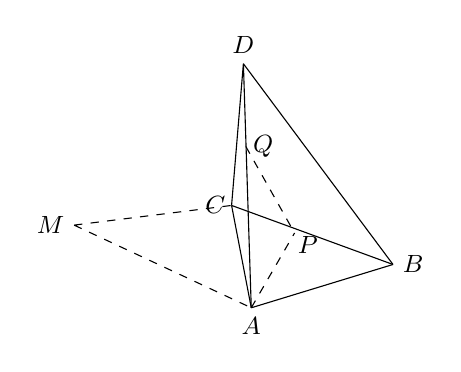
\begin{tikzpicture}[scale=1.0, font=\small]
  \coordinate (A) at (2.6,0);
  \coordinate (B) at (4.4,0.55);
  \coordinate (C) at (2.35,1.3);
  \coordinate (M) at (0.35,1.05);
  \coordinate (D) at (2.5,3.1);
  \coordinate (Q) at (2.53,2.05);
  \coordinate (P) at (3.15,0.95);
  \draw (A) -- (B);
  \draw (A) -- (C)  (B) -- (C);
  \draw (C) -- (D)  (A) -- (D);
  \draw (D) -- (B);
  \draw[dashed] (M) -- (A)  (M) -- (C);
  \draw[dashed] (A) -- (P)  (Q) -- (P);
  \node[below] at (A) {$A$};
  \node[right] at (B) {$B$};
  \node[left, inner sep=2pt] at (C) {$C$};
  \node[left] at (M) {$M$};
  \node[above] at (D) {$D$};
  \node[right, inner sep=2.5pt] at (Q) {$Q$};
  \node[below right, inner sep=1pt] at (P) {$P$};
\end{tikzpicture}
\end{center}

  (1) 证明：平面 $ACD\perp$ 平面 $ABC$；

  (2) $Q$ 为线段 $AD$ 上一点，$P$ 为线段 $BC$ 上一点，且 $BP=DQ=\dfrac23DA$，求三棱锥 $Q\text{-}ABP$ 的体积。

\gkti{19}\textbf{（12 分）} 某家庭记录了未使用节水龙头 $50$ 天的日用水量数据（单位：$\mathrm m^{3}$）和使用了节水龙头 $50$ 天的日用水量数据，得到频数分布表如下：

\textbf{未使用节水龙头 50 天的日用水量频数分布表}

\begin{center}
\begin{tabular}{cccccccc}
\toprule
日用水量 & $[0,0.1)$ & $[0.1,0.2)$ & $[0.2,0.3)$ & $[0.3,0.4)$ & $[0.4,0.5)$ & $[0.5,0.6)$ & $[0.6,0.7)$ \\
\midrule
频数 & $1$ & $3$ & $2$ & $4$ & $9$ & $26$ & $5$ \\
\bottomrule
\end{tabular}
\end{center}

\textbf{使用了节水龙头 50 天的日用水量频数分布表}

\begin{center}
\begin{tabular}{ccccccc}
\toprule
日用水量 & $[0,0.1)$ & $[0.1,0.2)$ & $[0.2,0.3)$ & $[0.3,0.4)$ & $[0.4,0.5)$ & $[0.5,0.6)$ \\
\midrule
频数 & $1$ & $5$ & $13$ & $10$ & $16$ & $5$ \\
\bottomrule
\end{tabular}
\end{center}

  (1) 在答题卡上作出使用了节水龙头 $50$ 天的日用水量数据的频率分布直方图：

\begin{center}% 2018 全国Ⅰ卷 文19：供作图用的空白频率分布直方图坐标网格
\begin{tikzpicture}
\begin{axis}[width=9.5cm, height=8cm, font=\small,
  xlabel={日用水量/$\mathrm{m}^{3}$}, ylabel={频率/组距},
  xlabel style={at={(1,0)}, anchor=west, font=\small},
  ylabel style={at={(0,1)}, anchor=south, rotate=-90, font=\small},
  xmin=0, xmax=0.65, ymin=0, ymax=3.5,
  xtick={0,0.1,...,0.6},
  ytick={0.2,0.4,...,3.4},
  yticklabel style={/pgf/number format/fixed, /pgf/number format/precision=1},
  xticklabel style={/pgf/number format/fixed, /pgf/number format/precision=1},
  grid=both, grid style={dashed, gray!45},
  axis lines=left, axis line style={-Stealth}]
\end{axis}
\end{tikzpicture}
\end{center}

  (2) 估计该家庭使用节水龙头后，日用水量小于 $0.35\ \mathrm m^{3}$ 的概率；

  (3) 估计该家庭使用节水龙头后，一年能节省多少水？（一年按 $365$ 天计算，同一组中的数据以这组数据所在区间中点的值作代表。）

\gkti{20}\textbf{（12 分）} 设抛物线 $C:y^{2}=2x$，点 $A(2,0)$，$B(-2,0)$，过点 $A$ 的直线 $l$ 与 $C$ 交于 $M$，$N$ 两点。

  (1) 当 $l$ 与 $x$ 轴垂直时，求直线 $BM$ 的方程；

  (2) 证明：$\angle ABM=\angle ABN$。

\gkti{21}\textbf{（12 分）} 已知函数 $f(x)=a\mathrm e^{x}-\ln x-1$。

  (1) 设 $x=2$ 是 $f(x)$ 的极值点，求 $a$，并求 $f(x)$ 的单调区间；

  (2) 证明：当 $a\ge\dfrac1{\mathrm e}$ 时，$f(x)\ge0$。

\par\medskip

\gksubpart{（二）选考题：共 10 分，第 22、23 题任选一题作答}

\begin{gktip}
\textbf{ 现行考纲已取消选做题}，以下两题仅作历史资料保留。
\end{gktip}

\gkti{22}\textbf{（10 分）〔选修 4-4：坐标系与参数方程〕} （\textbf{已取消}）

在直角坐标系 $xOy$ 中，曲线 $C_1$ 的方程为 $y=k|x|+2$。以坐标原点为极点，$x$ 轴正半轴为极轴建立极坐标系，曲线 $C_2$ 的极坐标方程为 $\rho^{2}+2\rho\cos\theta-3=0$。

  (1) 求 $C_2$ 的直角坐标方程；

  (2) 若 $C_1$ 与 $C_2$ 有且仅有三个公共点，求 $C_1$ 的方程。

\gkti{23}\textbf{（10 分）〔选修 4-5：不等式选讲〕} （\textbf{已取消}）

已知 $f(x)=|x+1|-|ax-1|$。

  (1) 当 $a=1$ 时，求不等式 $f(x)>1$ 的解集；

  (2) 若 $x\in(0,1)$ 时不等式 $f(x)>x$ 成立，求 $a$ 的取值范围。

\par\medskip

